A partir de los \textbf{requisitos de información} definidos en la \autoref{sec:InformationRequirements}, se ha elaborado el \textbf{modelo conceptual de datos} del sistema. Para mejorar su legibilidad, el modelo se presenta por módulos funcionales y no como un único diagrama global excesivamente denso.

Los diagramas de esta sección abstraen el \textbf{modelo físico de base de datos}: se mantienen las entidades, atributos relevantes y relaciones principales, pero se omiten tipos \textit{SQL}, claves técnicas y restricciones de implementación. Esta separación permite que el modelo conceptual explique el \textbf{dominio del problema}, mientras que el diseño físico detallado se desarrolla posteriormente en la arquitectura de almacenamiento.

\subsection{Modelo conceptual de datos M1}

El módulo \texttt{M1} modela el \textbf{acceso al sistema}, el \textbf{alta controlada de usuarios} y la trazabilidad de sesiones y acciones administrativas. La Figura~\ref{fig:mcd-m1} recoge las entidades principales de este bloque.

\begin{figure}[H]
    \centering
    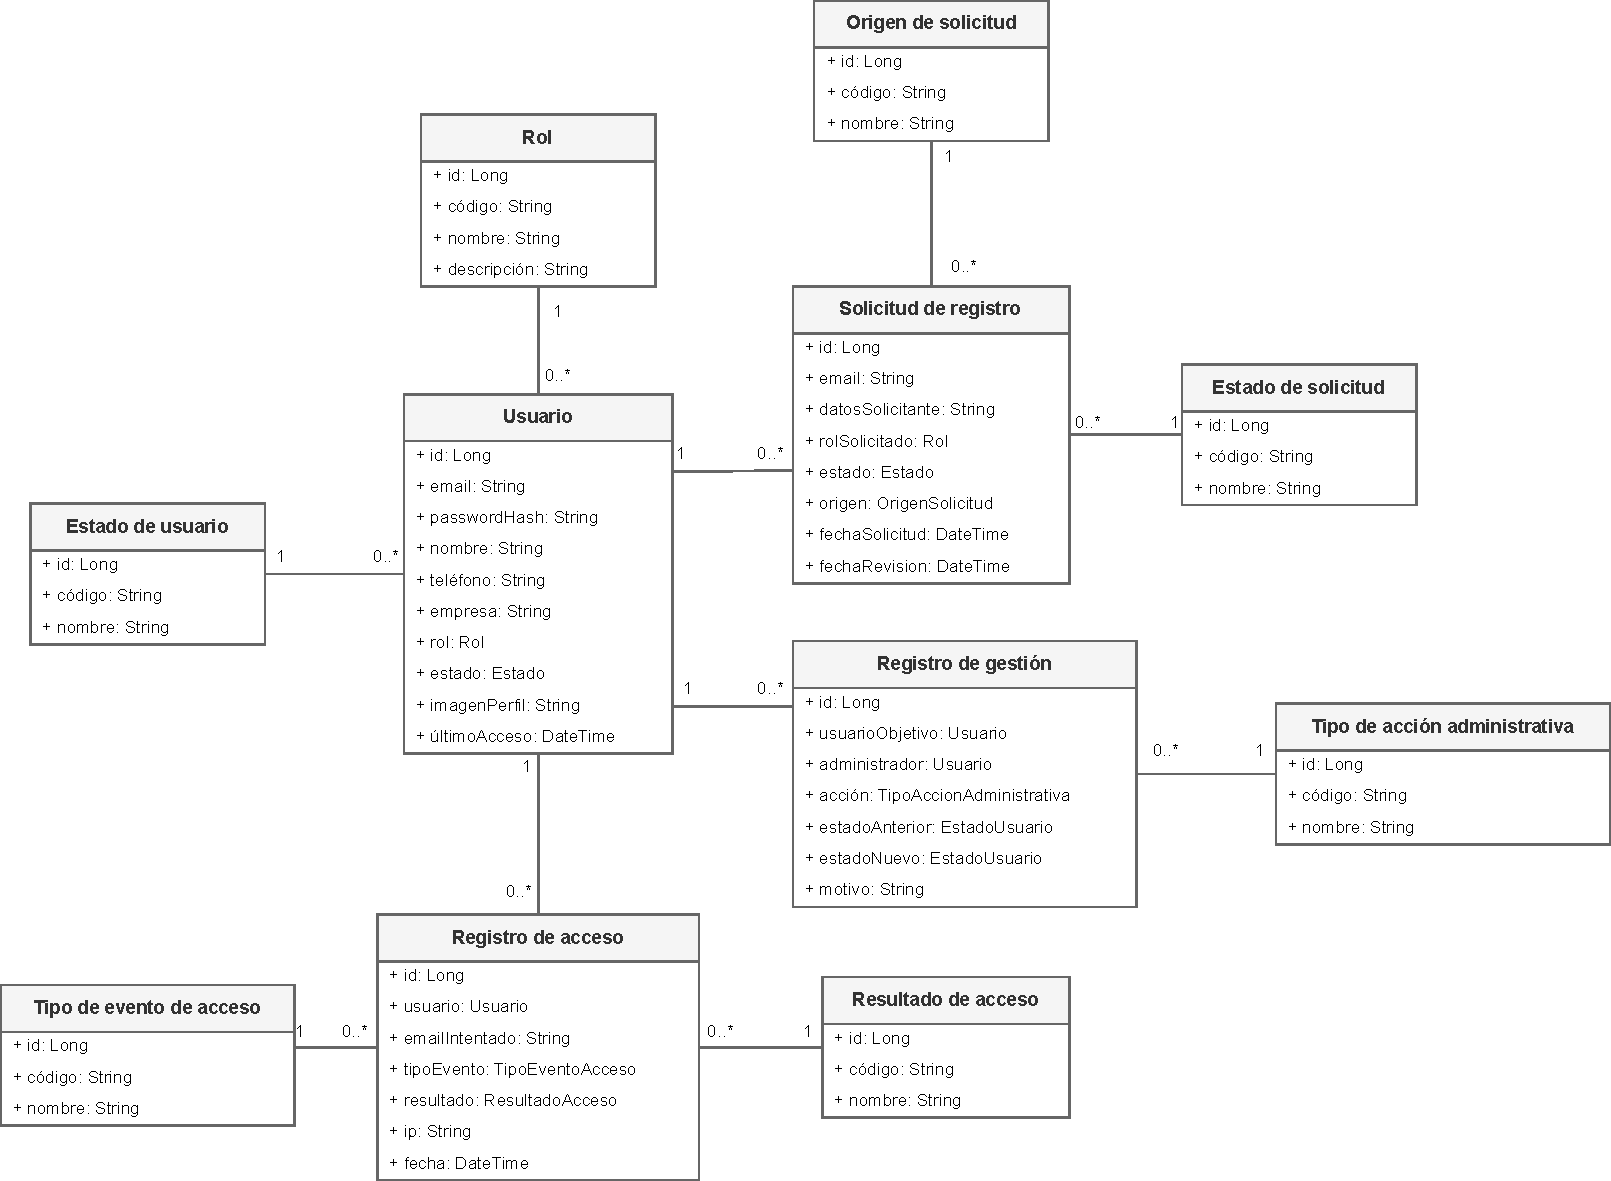
\includegraphics[width=\textwidth,height=0.65\textheight,keepaspectratio]{./figures/UML/MCD/M1_MCD_conceptual.pdf}
    \caption{Modelo conceptual de datos del módulo M1: acceso, usuarios y auditoría}
    \label{fig:mcd-m1}
\end{figure}

\subsection{Modelo conceptual de datos M2}

El módulo \texttt{M2} recoge la información necesaria para gestionar \textbf{clientes profesionales}, \textbf{comerciales}, asignaciones, visitas y rutas. La Figura~\ref{fig:mcd-m2} muestra la estructura conceptual de este módulo.

\begin{figure}[H]
    \centering
    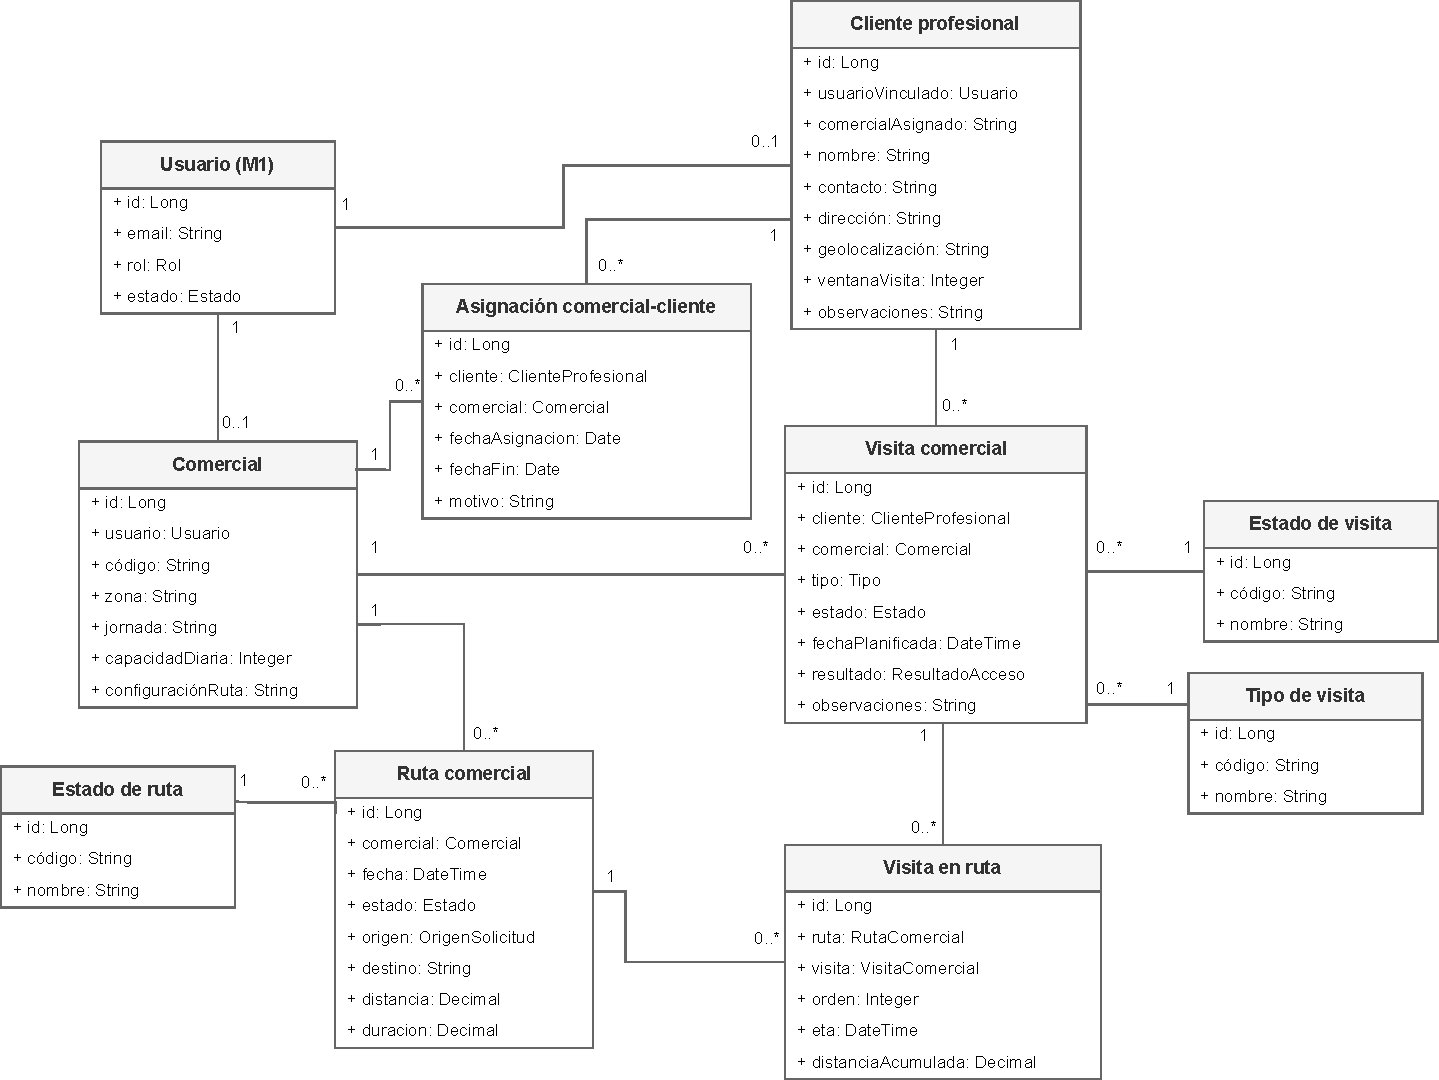
\includegraphics[width=\textwidth,height=0.65\textheight,keepaspectratio]{./figures/UML/MCD/M2_MCD_conceptual.pdf}
    \caption{Modelo conceptual de datos del módulo M2: clientes, comerciales, visitas y rutas}
    \label{fig:mcd-m2}
\end{figure}

\subsection{Modelo conceptual de datos M3}

El módulo \texttt{M3} representa el \textbf{catálogo de productos}, sus estructuras de clasificación, recursos de apoyo y cartas de color, incluyendo atributos comerciales como formato, embalaje, precio base y proveedor. La Figura~\ref{fig:mcd-m3} muestra las entidades y relaciones de este ámbito.

\begin{figure}[H]
    \centering
    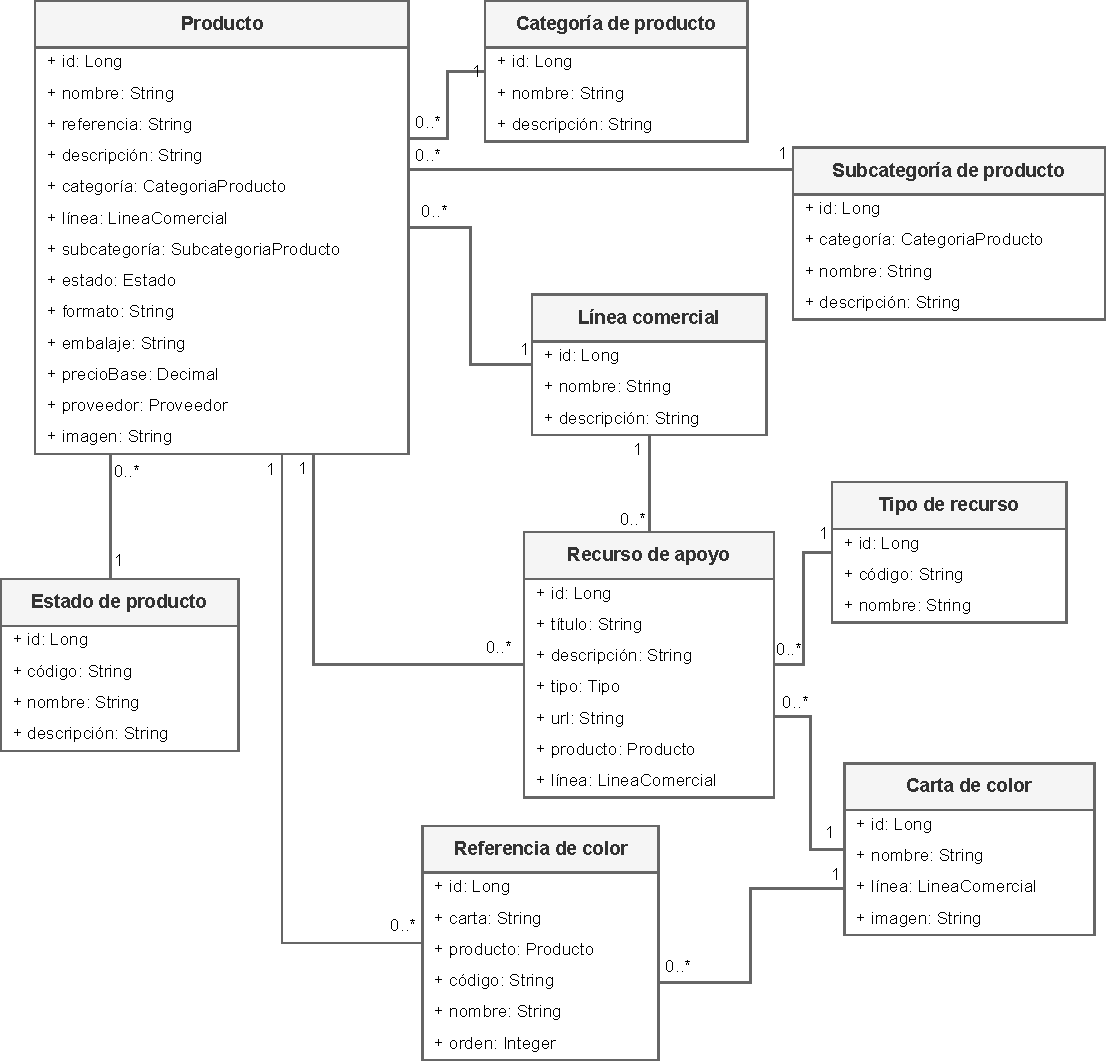
\includegraphics[width=\textwidth,height=0.65\textheight,keepaspectratio]{./figures/UML/MCD/M3_MCD_conceptual.pdf}
    \caption{Modelo conceptual de datos del módulo M3: catálogo, productos y coloración}
    \label{fig:mcd-m3}
\end{figure}

\subsection{Modelo conceptual de datos M4}

El módulo \texttt{M4} integra la \textbf{gestión de pedidos}, líneas, estados, preparación de repartos, validación de entrega y pagos asociados. En el modelo actual el pedido actúa como \textbf{cabecera comercial}, mientras que cada reparto representa una \textbf{unidad logística independiente} con bultos manuales, líneas servidas y etiqueta propia. La Figura~\ref{fig:mcd-m4} sintetiza este modelo conceptual actualizado.

\begin{figure}[H]
    \centering
    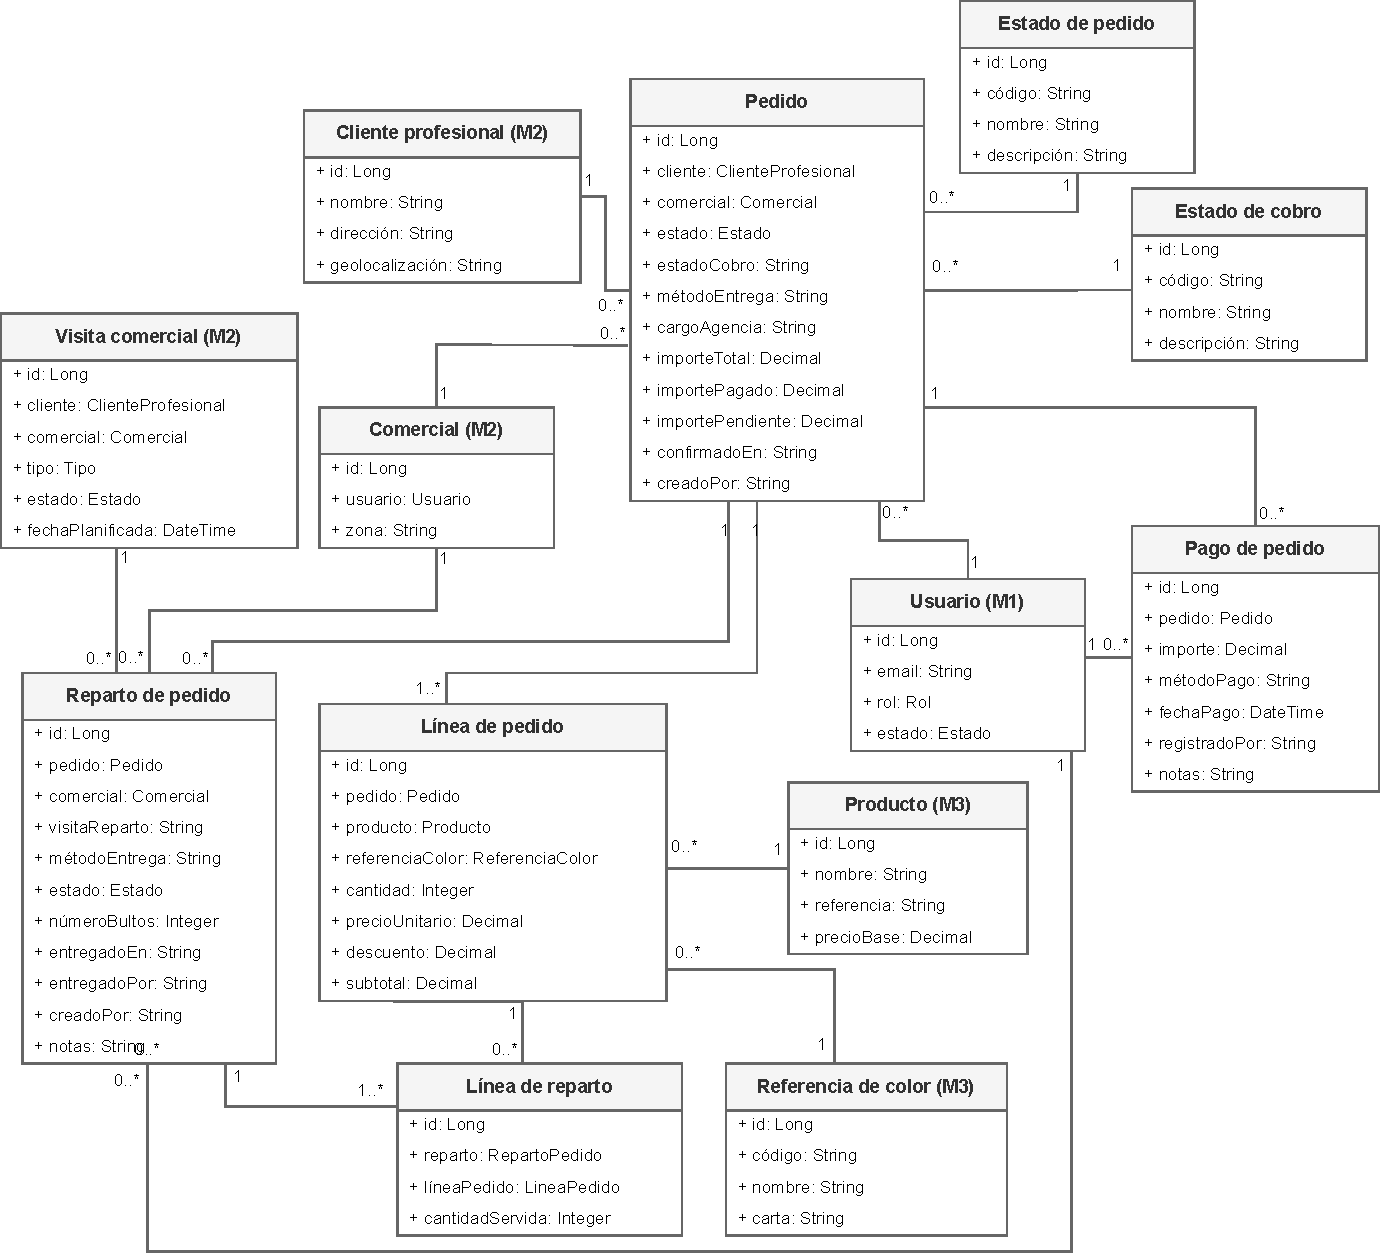
\includegraphics[width=\textwidth,height=0.65\textheight,keepaspectratio]{./figures/UML/MCD/M4_MCD_conceptual.pdf}
    \caption{Modelo conceptual de datos del módulo M4: pedidos, reparto y cobro}
    \label{fig:mcd-m4}
\end{figure}

\subsection{Modelo conceptual de datos M5}

El módulo \texttt{M5} modela la \textbf{gestión técnica del salón}: clientes finales, servicios realizados, fichas técnicas, productos utilizados, plantillas, imágenes y correos técnicos. La Figura~\ref{fig:mcd-m5} presenta las entidades principales de esta gestión.

\begin{figure}[H]
    \centering
    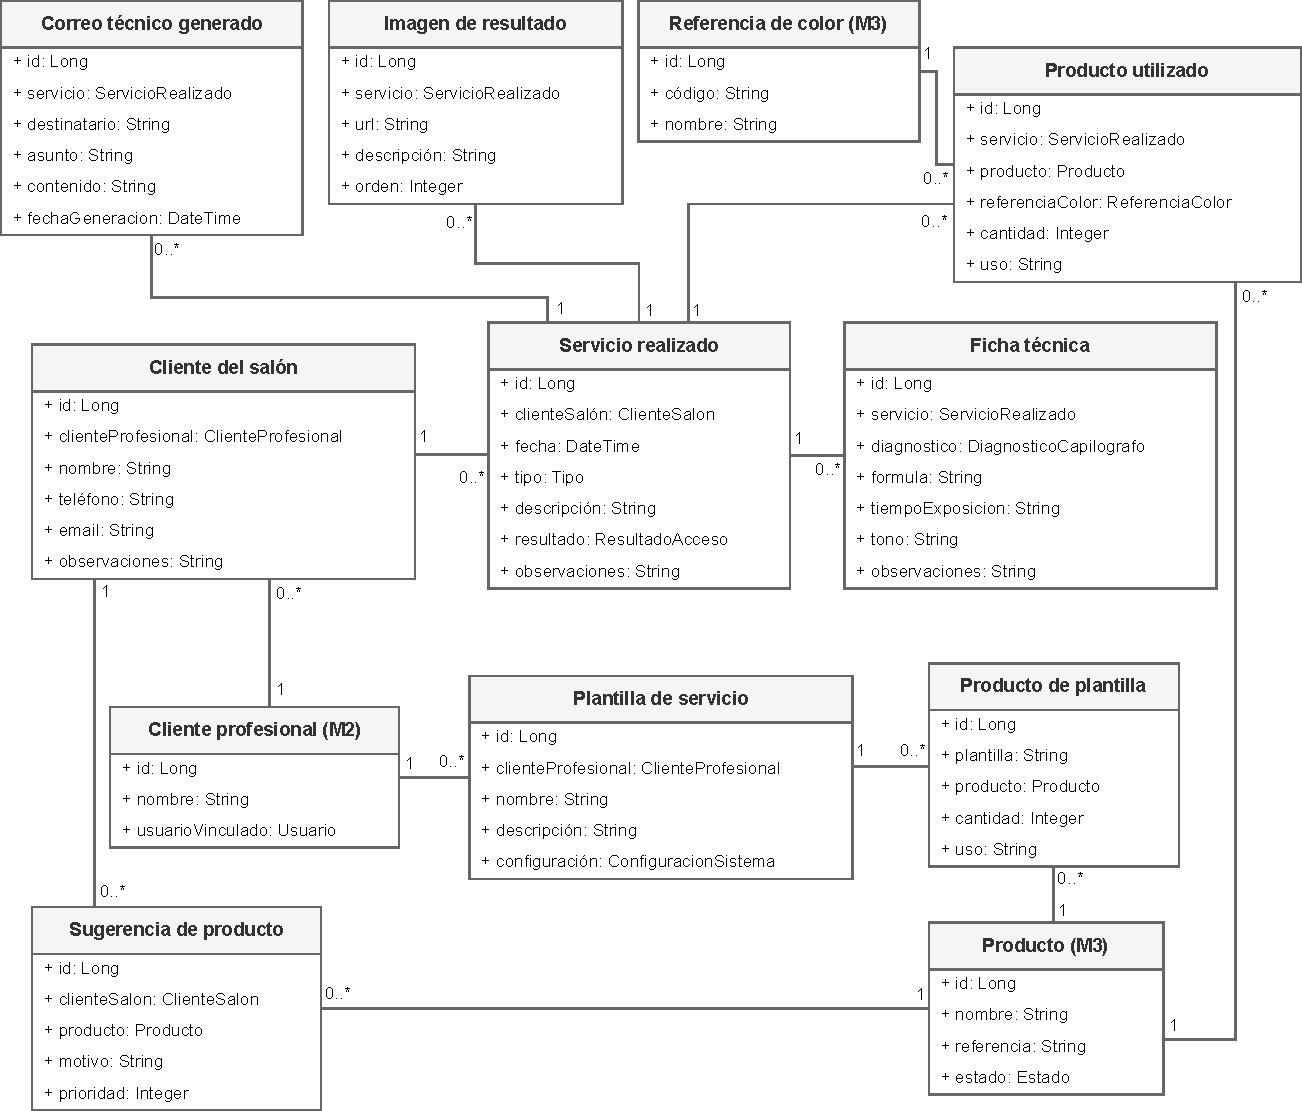
\includegraphics[width=\textwidth,height=0.65\textheight,keepaspectratio]{./figures/UML/MCD/M5_MCD_conceptual.pdf}
    \caption{Modelo conceptual de datos del módulo M5: gestión técnica del salón}
    \label{fig:mcd-m5}
\end{figure}

\subsection{Modelo conceptual de datos M6}

El módulo \texttt{M6} concentra \textbf{promociones}, tipos de promoción, segmentos de cliente, notificaciones, recordatorios, formaciones, inscripciones y soporte \textit{Web Push} \citep{webpushapi2026}. La Figura~\ref{fig:mcd-m6} recoge su estructura conceptual. En la implementación actual, la entidad de promoción se ha ampliado con adjuntos comerciales, tipo estructurado de descuento, porcentaje, umbral de volumen y regalo asociado; la \textbf{política de recálculo de rangos} se guarda como configuración transversal del módulo \texttt{M7}.

\begin{figure}[H]
    \centering
    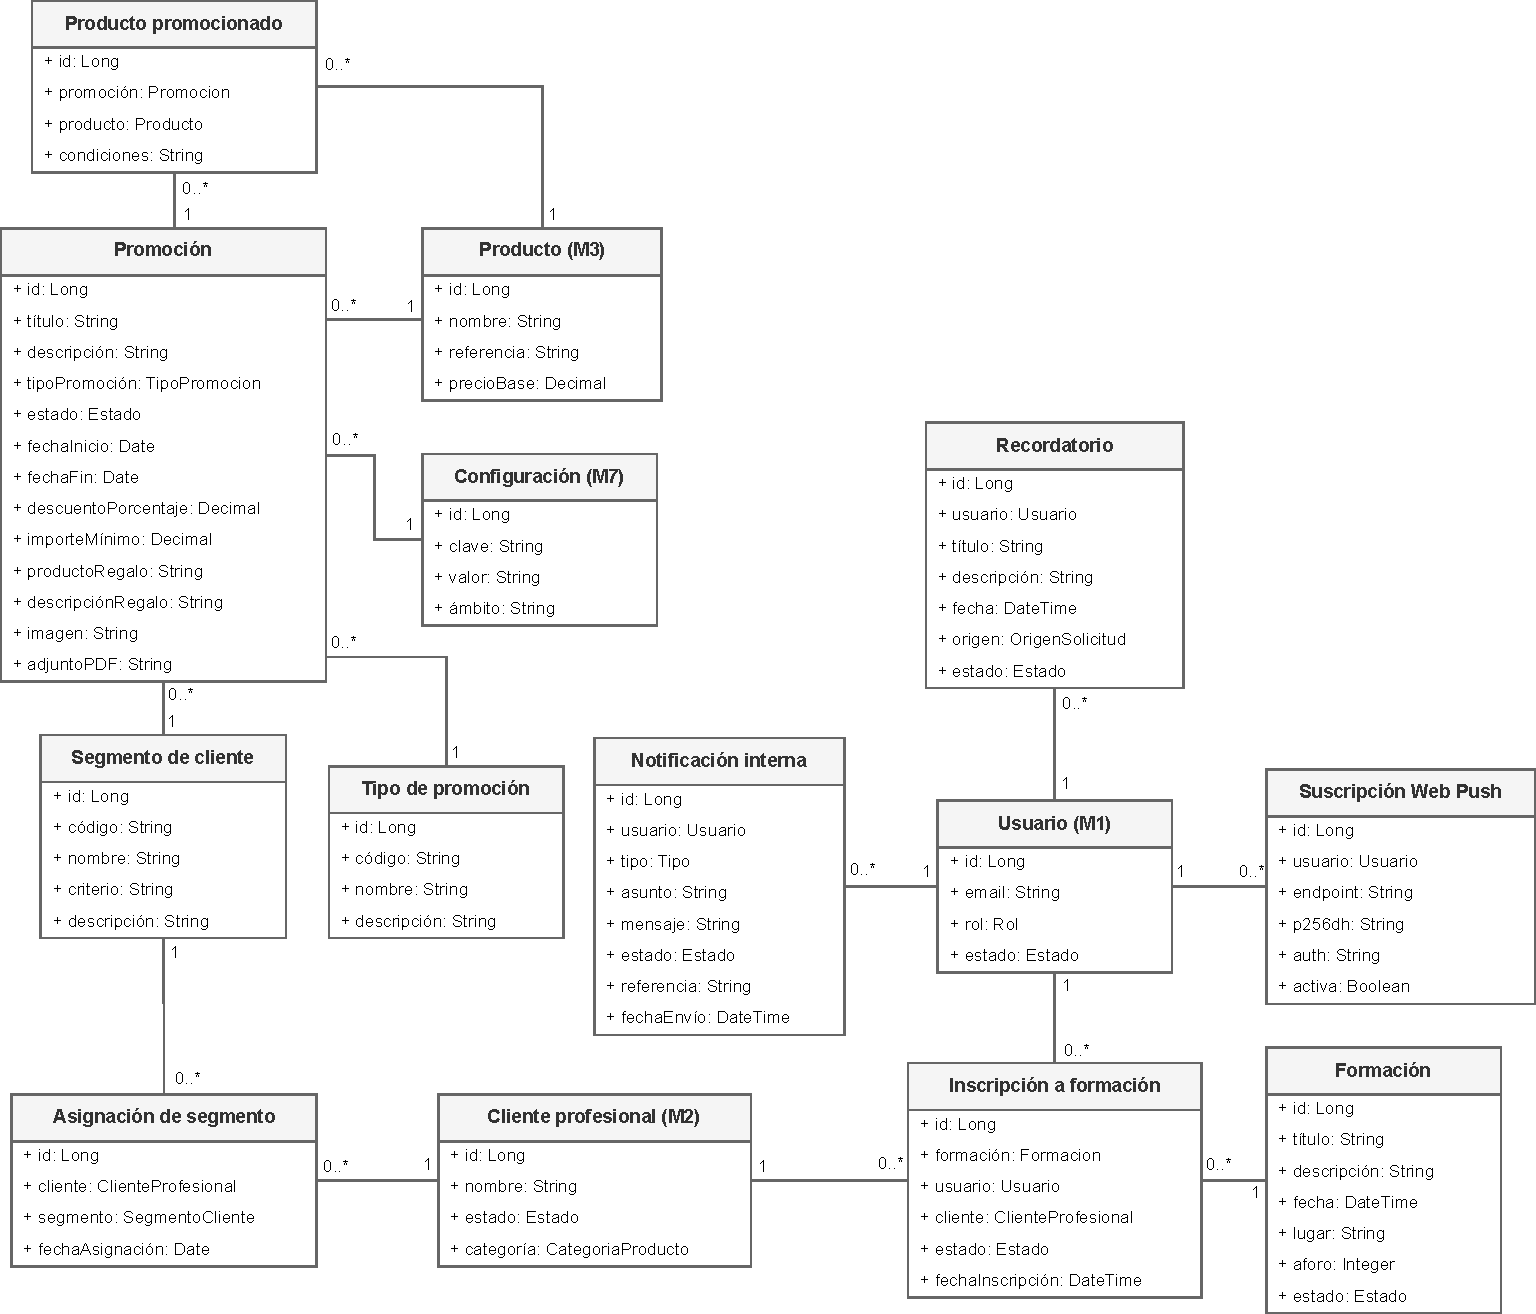
\includegraphics[width=\textwidth,height=0.65\textheight,keepaspectratio]{./figures/UML/MCD/M6_MCD_conceptual.pdf}
    \caption{Modelo conceptual de datos del módulo M6: comunicaciones, promociones y formación}
    \label{fig:mcd-m6}
\end{figure}

\subsection{Modelo conceptual de datos M7}

El módulo \texttt{M7} cubre la \textbf{administración transversal}: configuraciones del sistema, políticas de limitación, servicios auxiliares, registros técnicos y propuestas internas de pedido a proveedor. La Figura~\ref{fig:mcd-m7} muestra el modelo conceptual de este bloque transversal.

\begin{figure}[H]
    \centering
    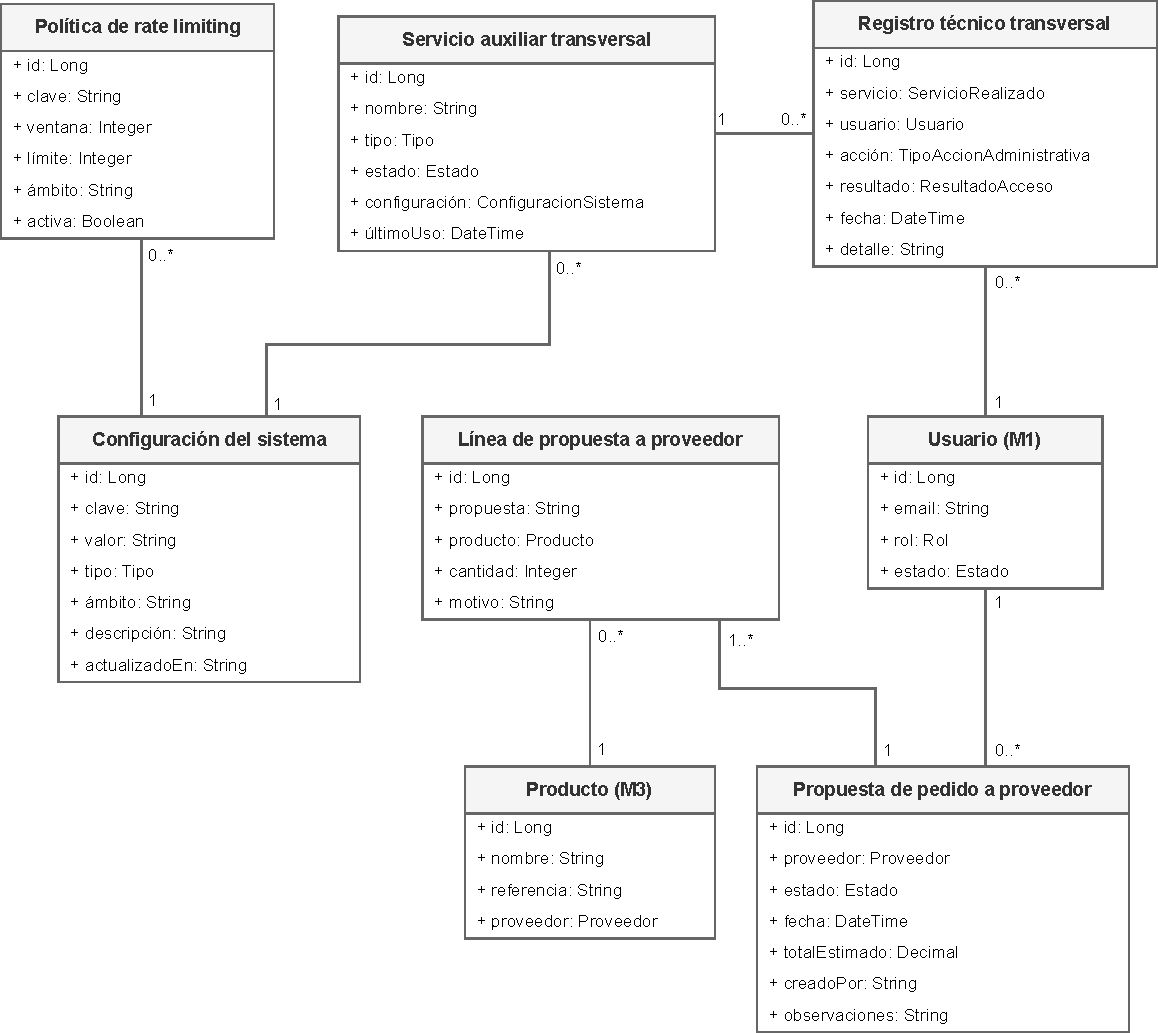
\includegraphics[width=\textwidth,height=0.65\textheight,keepaspectratio]{./figures/UML/MCD/M7_MCD_conceptual.pdf}
    \caption{Modelo conceptual de datos del módulo M7: administración transversal}
    \label{fig:mcd-m7}
\end{figure}

\subsection{Modelo conceptual de datos M8}

El módulo \texttt{M8} representa \textbf{funcionalidades previstas para evolución futura}, como diagnóstico capilar con capilógrafo e inteligencia artificial, simulación de estilo o coloración mediante cámara móvil, reconocimiento de productos, reserva \textit{online}, asistente virtual tipo \textit{chatbot} y automatización de servicios externos como Factusol mediante \textit{n8n} o \textit{APIs} equivalentes \citep{sdelsol-factusol,n8n-webhook,n8n-http-request}. La Figura~\ref{fig:mcd-m8} deja identificadas sus necesidades de información principales, aunque no forma parte del alcance implementado principal.

\begin{figure}[H]
    \centering
    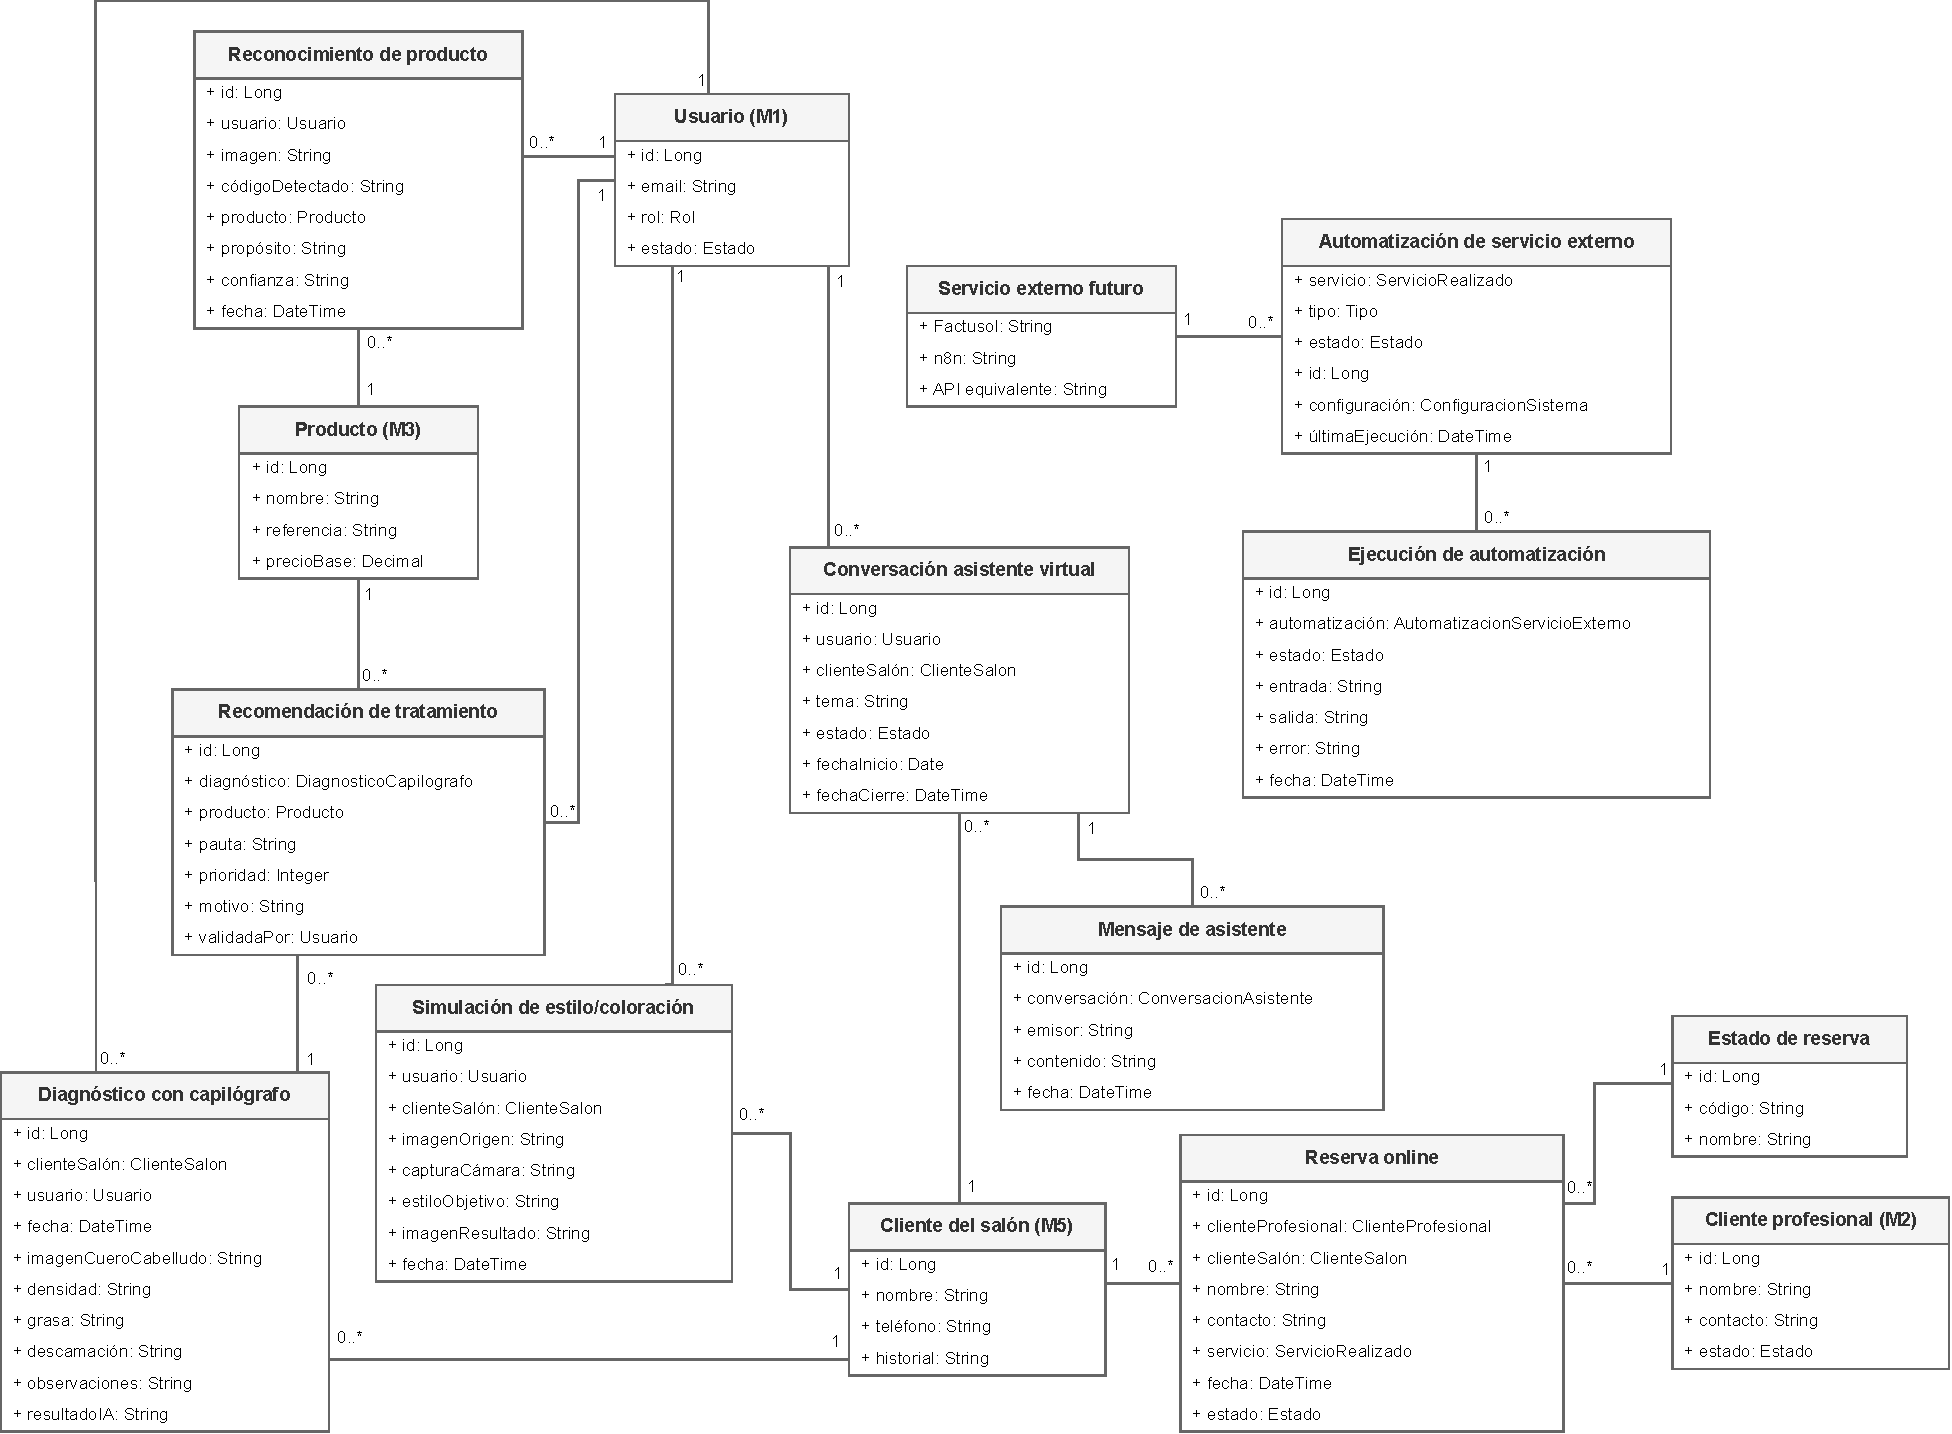
\includegraphics[width=\textwidth,height=0.65\textheight,keepaspectratio]{./figures/UML/MCD/M8_MCD_conceptual.pdf}
    \caption{Modelo conceptual de datos del módulo M8: funcionalidades inteligentes previstas}
    \label{fig:mcd-m8}
\end{figure}
